% !TEX root = sum1.tex
\section{Dynamic demand situation}\label{dynamic_demand}

We also study the dynamic seating plan problem, which is more suitable for commercial use. In this situation, customers come dynamically, and the seating plan needs to be made without knowing the number and composition of future customers. 

It becomes a sequential stochastic optimization problem where conventional methods fall into the curse of dimensionality due to many seating plan combinations. To avoid this complexity, we develop an approach that aims directly at the final seating plans. Specifically, we define the concept of target seating plans deemed satisfactory. In making the dynamic seating plan, we will try to maintain the possibility of achieving one of the target seating plans as much as possible.

\subsection{Dynamic Situation without Stochastic Information}

\subsection{Solve the dynamic situation with the largest patterns}\label{largest_pattern}

Partially dynamic: at the beginning stage, the capacity is sufficient, thus we will accept all arrivals. Suppose that we don't know the stochastic information, we can use the multiple planning approach (Apply the largest pattern for each row). 
When the largest patterns cannot accept more groups, we can change the 
largest pattern to a second largest pattern according to the realized arrivals.

% There is a reservation stage, we only decide to accept or reject.

% After certain periods, there is a seat selection stage.

When we have the stochastic information, we can use nested policy based on the multiple planning approach. 
For each row, we can choose the pattern from $I_1$. Accept the group such that the largest pattern can be maintained. When the arrival cannot be assigned in the planning patterns from $I_1$, we use the nested policy to make the decision. 

% Or use partial static information to estimate the probabilities, then generate new plannings.

% Multiple scenario approach:
% Suppose that we know the probabilities, we can use the sampling demands to estimate which patterns we should use. For example, three rows with $I_1$, seven rows with $I_2$. For each arrival, if there exists one scenario containing this group, we accept it; otherwise we use nested policy to accept or reject it.

\begin{algorithm}[H]\label{algo_largest}
  \caption{Method by using the largest patterns}
  \begin{description}
    \item[Step 1.] Generate the largest pattern by the greedy way for each row.
    \item[Step 2.] Denote the minimal and maximal size of group in the pattern of row $i$ as $\min_i$ and $\max_i$. 
    \item[Step 3.] For the arrival with the size of $a$ in period $t$, if there exists $i$ such that $\min_i + \max_i >= a$ and $a > \min_i$, accept this arrival at row $i$ and go to step 5; otherwise, go to step 4.
    \item[Step 4.] Add up the remaining supply for all rows, use the nested policy to make the decision.
    \item[Step 5.] Move to the next period. Repeat step 3. 
  \end{description}
\end{algorithm}

Step 2: the pattern will have the same loss by these procedures. ($\min_i$ can be 0.)

\begin{lem}
  Any largest patterns can be generated by the largest pattern constructed from the greedy method.
\end{lem}

Results compared with other methods:

We can compare M3 with M5, the improvement from M3 to M5 results from the stochastic information. But the result of M5 is not ideal compared with other methods.

M3 can be used without stochastic information.


\subsection{Generate Scenarios with Stochastic Information}\label{MappingSeq}

At first, we can use the stochastic information to generate scenarios.

% Fix the supply of this group size, and continue this procedure.  

% If groups arrive randomly, the procedure will be similar. 

% We don't care about the arrival sequence; only the number of groups matters. Because as long as the approximation about the number of groups is accurate, we can handle any sequence.

\subsubsection{Mapping sequences to scenarios by discrete periods}

Notice that this approach still works under the assumption that time is continuous.

Suppose there are $T$ independent periods, at most one group will arrive in each period.

There are $J$ different group types(including the group with no people). Let $\mathbf{y}$ be a discrete random variable indicating the number of people in the group. Let $\mathbf{p}$ be the vector probability, where $p(y = j) = p_j$, $j = 0,1,\ldots,J-1$ and $\sum_{j} p_{j} =1$. Then a sequence can be expressed as $\{y_{1}, y_{2}, \ldots, y_{T}\}$. (It can be modeled as a multinomial distribution, $p(\mathbf{Y} \mid \mathbf{p})=\prod_{j=0}^{J-1} p_j N_j$).

Let $N_{j} = \sum_{t} I(y_t = j)$, i.e., the count number of times group type $j$ arrives during $T$ periods. Then the set of counts $N_{j}$ (scenarios) follows a multinomial distribution, $$p\left(N_0, \ldots, N_{J-1} \mid \mathbf{p}\right)=\frac{T !}{N_{0}!, \ldots, N_{J-1}!} \prod_{j=0}^{J-1} p_{j}^{N_j}, T = \sum_{j=0}^{J-1} N_{j}$$

% scenario:

% sequence will affect the result.
% Then, if we fix the seat assignment as $[3,3]$. For the sequence, $2,2,2,2,2,3,3,3,3,3$, we will place one $2$ in a three-seat. 
% But for the sequence, $3,3,3,3,3,2,2,2,2,2$, we will accept three $3$ and three $2$.

Show the complexity: the number of different sequences $J^{T}$, and the number of scenarios is $O(T^{J-1})$.

Obtained by DP:
Use $D(T,J) $ to denote the number of scenarios, which equals to the number of different solutions to $x_{1}+\ldots + x_{J} = T, \mathbf{x} \geq 0$.
Then we know the recursion relation $D(T, J) = \sum_{i= 0}^{T} D(i, J-1)$ and $D(i,2) = i+1, D(i,1) = 1$.
$D(T,3) = \frac{(T+2)(T+1)}{2}, D(T,J) = O(T^{J-1})$.

The number of scenarios is too large to enumerate all possible cases.
Thus, we choose to sample some sequences from the multinomial distribution.


% Example:
% The group types are $[2,3,4,5]$. The number of periods is $20$. The number of given rows is 4 and the number of seats is 22.
% Each group arrives with the same probability.
% The number of sequences generating from multinomial distribution is $1000$. Then, we can obtain $[0,3,6,11]$ from stochastic programming. When the number of sequences is 5000, we still obtain $[0,3,6,11]$. It shows that sampling is practical.

\subsubsection{Mapping sequences to scenarios by continuous time}

When the time is continuous, we only need to count the number of different group types, the method will be the same.

For the nonhomogeneous Poisson process, $N_{i}(T) \sim Poisson (\int_0^{T} p_i(s)\lambda(s) \mathrm{d} s)$. If the Poisson process is homogeneous, $N_{i} \sim Poisson(\lambda p_i T)$ during the interval $[0, T]$. Then for a realization of the Poisson process, we can still apply the method in Section \ref{MappingSeq}.

\subsection{Nested policy when given supply}\label{nested_policy}
% Recall that the stochastic programming only considers the situation that small-size groups can use the surplus large-size seats.

Once we obtain a solution from the stochastic programming, we need to follow some basic rules to assign the seats.
\begin{itemize}
    \item When the supply of one arriving group is enough, we will accept the group directly.
    \item When the supply of one arriving group is 0, the demand can be satisfied by only one larger-size supply.
    \item When one group is accpected to occupy the larger-size seats, the rest empty seat(s) can be reserved for the future demand.
\end{itemize}

we can assign the seats to the corresponding-size group. But when a group comes while the corresponding supply is 0, should we assign this group to the larger-size seats? Now we demonstate the nested policy for this problem.

If we accept a group of $i$ to take over $j$-size seats, then the expected served people is $i + (j-i-1)P(D_{j-i-1} \geq x_{j-i-1}+1)$, where $i < j$, $P(D_i \geq x_i)$ is the probability of that the expected demand of group type $i$ in the following periods is no less than $x_i$, the remaining supply of group type $i$.

When a group of $i$ occupies $j$-size seats, $(j-i-1)$ seats can be provided for one group of $j-i-1$ with one seat of social distancing.
Thus, $P(D_{j-i-1} \geq x_{j-i-1}+1)$ indicates the probability of that the demand of group type $(j-i-1)$ in the future is no less than its current remaining supply plus 1. If $j -i-1 =0$, then this term equals 0.

Similarly, when the expected demand of group of $j$ in the future is no less than its remaining supply currently, we would reject a group of $i$, the expected served people is $j P(D_{j} \geq x_{j})$.

Let $d(i,j)$ be the difference of expected served people between acceptance and rejection on group $i$ occupying $j$-size seats. Then $d(i,j) = i + (j-i-1)P(D_{j-i-1} \geq x_{j-i-1}+1) - j P(D_{j} \geq x_{j}), j >i$.

One intuitive decision is to choose the largest difference.

We can obtain $d(i,j) = j P(D_{j} \leq x_{j} -1) - (j-i-1)P(D_{j-i-1} \leq x_{j-i-1}) -1$ after reformulating. 
Let $F_{j}(x;T)$ be the cumulative distribution function of the number of arrival groups $D_{j}$ in $T$ periods. Then $F_{j}(x; T_{r}) = P(D_{j} \leq x)$, and $D_{j}$ follows a binomial distribution $B(T_{r}, p_{j})$, where $T_{r}$ is the numebr of remaining periods.

Thus, $d(i,j) = j F_{j}(x_{j}-1; T) - (j-i-1) F_{j-i-1}(x_{j-i-1}; T) -1$. For all $j >i$, find the largest $d(i,j)$, denoted as $d(i,j^{*})$.

If $d(i,j^{*}) >0$, we will place the group $i$ in $j^{*}$-size seats. Otherwise, the group will be rejected.

The algorithm is shown below:

\begin{algorithm}[H]
  \caption{Nested policy under given supply}\label{algo_nested_policy}
  \begin{description}
    \item[Step 1.] Obtain a supply, $\X^{0} = [x_1,\ldots,x_{J}]$, from the stochastic programming.
    \item[Step 2.] For the arrival group type $i$ at period $T{'}$, if $x_{i} > 0$, accept it. Let $x_{i} = x_{i} -1$. Go to step 4.
    \item[Step 3.] If $x_{i} = 0$, find $d(i,j^{*})$. If $d(i,j^{*})>0$, accpect group type $i$. Set $x_{j^{*}} = x_{j^{*}} -1$. Let $x_{j-i-1} = x_{j-i-1} + 1$ when $j-i-1>0$. If $d(i,j^{*}) \leq 0$, reject group type $i$.
    \item[Step 4.] If $T{'} \leq T$, move to next period, set $T{'} = T{'}+1$, go to step 2.
  \end{description}
\end{algorithm}

% Example:

% If the supply is $[0,3,6,11]$, then here comes a group of 1. There will be three choices.
% \begin{align*}
% 1 \geq 2 P(D_{2} & \geq x_{2}) \\
% 1 + 1\cdot P(D_{1}\geq 1) & \geq 3 P(D_{3}\geq x_{3}) \\
% 1 + 2\cdot P(D_{2}\geq (1+ x_{2})) & \geq 4 P(D_{4}\geq x_{4})
% \end{align*}
% $\mathbf{x}$ is the remaining supply right now.

We show the results of Benders and IP under nested policy in section \ref{Bender_IP}.


\subsection{Seat assignment scenarios and methods}
In this section, we will present several methods to assign seats under different scenarios.

At first, we give the general method to deal with the dynamic situation.

\begin{algorithm}[H]\label{general_method}
  \caption{General method to deal with the Dynamic situation}
  \begin{description}
    \item[Step 1.] Obtain a linear solution from stochastic programming \eqref{BD_master1}.
    \item[Step 2.] Obtain the near-optimal integral solution from deterministic model with lower and upper bounds.
    \item[Step 3.] Accept or reject group arrivals according to the nested policy in section \ref{nested_policy}.
    \item[Step 4.] According to different scenarios, we can fix the supply or re-calculate to give a new supply. 
    % update the scenario and the probability, add constraints when re-calculating stochastic programming.
    % we can update the supply whenever some demand exceeds the supply.
  \end{description}
\end{algorithm}

In step 4, the scenarios include the ticket reservation without seat selection, ticket reservation with only row selection, ticket reservation with restricted seat selection. 

% Different methods are derived to deal with these situations. 

These senarios are described as follows:

1. Seat assignment will not be made immediately, we only need to reject or accept each request during the making-reservation stage. After the deadline of the reservation, we will give the seat assignment and tell the groups their seats when they check in. This scenario applies for the reservation without seat selection. For example, some theaters and concerts only provide the seat reservation for the audiences.

2. The groups can only choose which row to sit. This scenario appears in the on-site seminar. 

We need to assign seats to the group for each arrival. In each period, the group can select the row they want to sit when the capacity is enough. 

FCFS will be more appropriate. But M1 and M3 can also be used.

% After certain periods, we update the remaining seats in each row. have a row list, used for M2.  

3. Online booking. (Can select arbitrarily but with some constraints.)

When the customers book the tickets, they will be asked how many seats they are going to book at first. Then we give the possible row numbers for their selection. Finally we give the seat number for their choice.

The second step is based on the other choices of reserved groups, we need to check which rows in the seat assignment include the corresponding-size seats.

In third step, we need to check whether the chosen number destroys the pattern of the row. Use subset sum problem to check every position in the row.

% 1.2 Every group can choose where to sit according to the assignment.
% In each period, every group can choose to sit everywhere as long as the assignment allows. If one group choose to sit in the middle of some row, then this row is divided into two rows. 
% After certain periods, we update the remaining seats and rows, then solve a similar problem.

4. The seat assignment will be arranged before the arrival of groups, the groups only need to find the corresponding-size seats. This scenario applies for the reservation without seat selection. For example, the movie halls can assign the seats in advance to save costs. And seat assignment could be remained in one day because the same film genre will attract the same feature of different group types.


There are six methods basically:

M1: The seat assignment(supply) is obtained from stochastic model. Then use Algorithm \ref{algo_nested_policy} to make the decision.

M1 can be used in scenario 1,2,3,4. The seats can be placed in the cinema hall in advance.
% unsettle the useless seats.

M2: DP-based. We relax several rows to one row with the same capacity. Suppose there always exists one assignment under the capacity. Then we can use DP to make the decision in each period.

$$V(S,T) = \sum_{i \in N} p_i \max\{ {[V((S-s_i-1),T-1)+ s_i]}, {V(S,T-1)}\}$$

After obtaining the accpected sequence, we still need to check whether this sequence is feasible for the seat assignment. For most cases, it is feasible. That is the reason why we choose DP. When it is not feasible, we should delete the group one by one from the last arrival of the sequence until it is feasible.

In practice, we accept the request until we cannot find the seat assignment. It can only be applied in scenario 1.

% we can use a buffer to contain the accpected groups, when the groups can be assigned to a full row, then remove them from the buffer. 

% In fact, direct DP will have a gap, we should use a buffer to improve this method.

% For example, the number of seats for 10 rows is 21. The demand is $[1,2,41,16]$. The optimal assignment is $[0, 0, 40, 10]$. But DP will give $[0, 0, 35, 14]$.

% When a full pattern is reached, then delete the related groups and the row. Update the remaining demand.

% We know $(0,0,4,1)$ is a largest and full pattern, thus an assignment constructed with these 10 patterns is an optimal assignment.

M3: Set the largest pattern in each row. See section \ref{largest_pattern}

M4: 
The inital supply is obtained from stochastic model, update the supply from deterministic model by setting accpected demand as the lower bound. / It can be used in scenario 1,2. (The initial supply can be other demands.)

% Set the mean demand as the initial supply, update the supply from deterministic model by setting accpected demand as the lower bound. / can be used in scenario 1,2.

M5:
The intuitive but trivial method will be first-come-first-serve. Each request will be assigned row by row. When the capacity of one row is not enough for the request, we arrange it in the next row. If the following request can take up the remaining capacity of some row exactly, we place it in the row immediately. We check each request until the capacity is used up. 

It can be used in scenario 1,2,3. For scenario 3, the performane will be worse without restriction.

% Set the maximal people from the offline sequence.


M6: Based on first-come-first-serve. For the arrival sequence, find the target arrival when the total number of seats taken by the preceding arrivals does not exceed the capacity. And use nested policy to accept or reject one group in the remaining arrivals.

Then we obtain a new sub-sequence, which includes the arrivals from the first one to the target one and a possible arrival.

Similar to M2, when it is not feasible for the seat assignment, we should delete the group one by one from this sub-sequence until it is feasible.

It can be used in scenario 1. 

The relation between the scenarios and the methods is showed in the following table:
\begin{table}[ht]
  \centering
  \caption{Relation between the scenarios and the methods}
  \begin{tabular}{|l|l|l|l|l|l|l|}
  \hline
   & M1 & M2 & M3 & M4 & M5 & M6 \\
  \hline
  Scenario 1 & \checkmark & \checkmark & \checkmark & \checkmark & \checkmark & \checkmark \\
  Scenario 2 & \checkmark &            & \checkmark & \checkmark & \checkmark &            \\
  Scenario 3 & \checkmark &            & \checkmark &            & \checkmark &            \\
  Scenario 4 & \checkmark &            &            &            &            & \\
  \hline
  \end{tabular}
\end{table}


% Once: Obtain the supply from the stochastic model by benders decomposition. Use the deterministic model to obtain a heuristi supply. Then use the multi-class rule to decide whether to accept the group at each period.

% Several: Initially, set the mean demand for all periods as the upper bound of demand. Then obtain the supply from the deterministic model. Set the accepted demand as the lower bound of demand, the upper bound of demand will be the sum of accepted demand and mean demand for the remaining periods. Update the lower bound and upper bound when some supply runs out.

% One counterexample: [15,21,13,3] /[15,21,10,3]  reject 4

% Different types of movies will have different probabilities, consider the preference for policy when demand = supply.

The results of different methods on scenario 1 are shown below.

\begin{table}[ht]
  \begin{tabular}{|l|l|l|l|l|}
  \hline
  \# samples & T & probabilities & \# rows & performance(\%) compared to the optimal \\
  \hline
  1000  & 50  & [0.4,0.4,0.1,0.1] & 8 & (99.72, 100.00, 100.00, 100.00, 98.11, 100.00) \\
  1000  & 55  & [0.4,0.4,0.1,0.1] & 8 & (97.75, 99.83, 99.76, 99.76, 93.15, 99.76) \\ % slow
  1000  & 60  & [0.4,0.4,0.1,0.1] & 8 & (95.78, 99.20, 97.80, 97.80, 89.35, 97.65) \\
  1000  & 65  & [0.4,0.4,0.1,0.1] & 8 & (95.61, 99.10, 96.23, 96.23, 87.80, 96.12) \\
  \hline
  1000  & 40  & [0.25,0.25,0.25,0.25] & 8 & (99.94, 100.00, 100.00, 100.00, 98.22, 100.00) \\
  1000  & 45  & [0.25,0.25,0.25,0.25] & 8 & (97.19, 99.51, 99.09, 99.09, 91.31, 99.29) \\
  1000  & 50  & [0.25,0.25,0.25,0.25] & 8 & (95.23, 98.98, 97.21, 97.21, 87.73, 96.88) \\
  1000  & 55  & [0.25,0.25,0.25,0.25] & 8 & (94.84, 99.05, 95.70, 95.70, 85.49, 95.13) \\
  \hline
  \end{tabular}
\end{table}
 
The numbers in the `performance compared to the optimal' represent M1, M2, M3, M4, M5, M6 respectively in order.

The maximal number of people served can be obtained by \eqref{deter_upper} with a realized sequence of arrival.


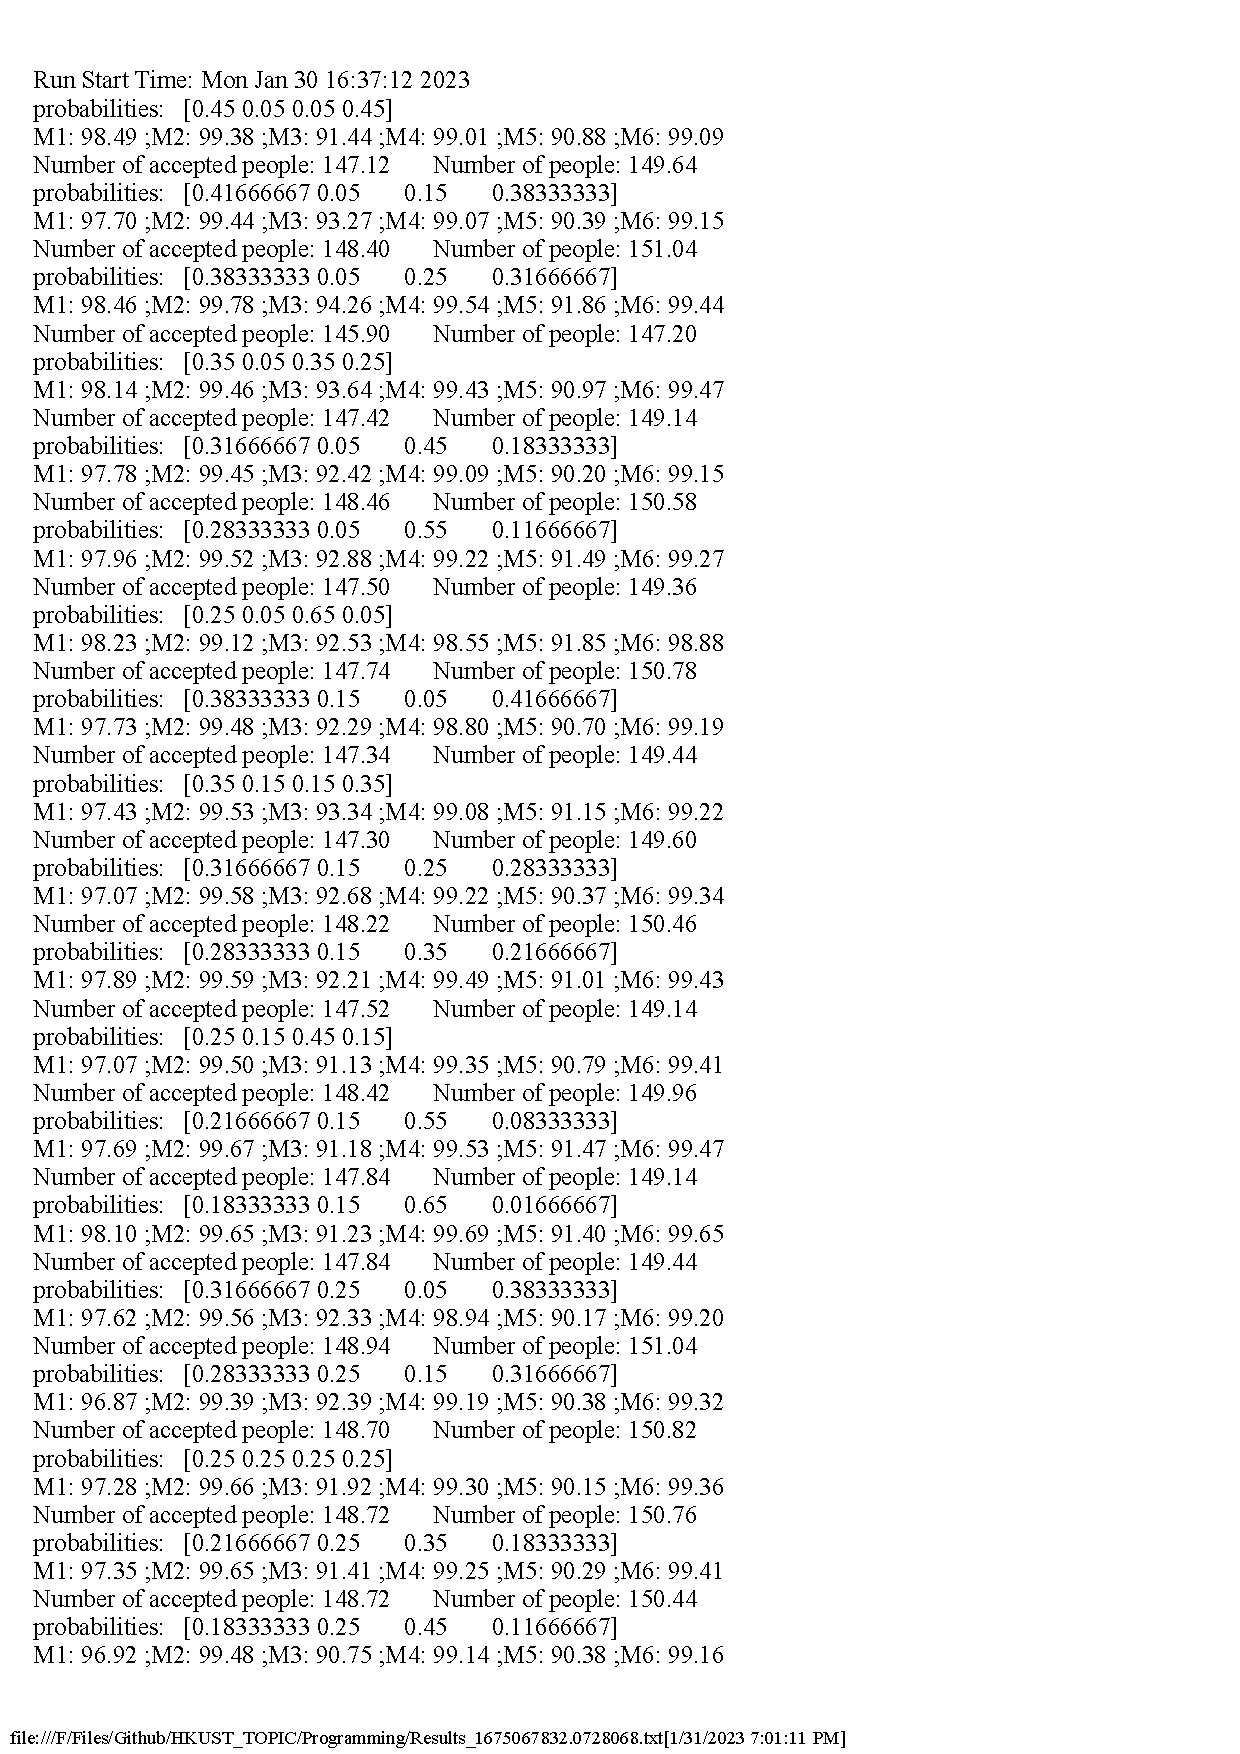
\includepdf{./Figures/Results_M3.pdf}